\documentclass[conference]{IEEEtran}
\IEEEoverridecommandlockouts
% The preceding line is only needed to identify funding in the first footnote. If that is unneeded, please comment it out.
\usepackage{cite}
\usepackage{amsmath,amssymb,amsfonts}
\usepackage{algorithmic}
\usepackage{graphicx}
\usepackage{url}
\usepackage[utf8]{inputenc}
\usepackage{textcomp}
\usepackage{multirow}
\usepackage{booktabs}
\usepackage{subfig}
\usepackage{nameref}

\usepackage[english,ngerman,brazilian]{babel}
\def\BibTeX{{\rm B\kern-.05em{\sc i\kern-.025em b}\kern-.08em
    T\kern-.1667em\lower.7ex\hbox{E}\kern-.125emX}}
\begin{document}

\title{Projeto Final - UNBeauty: Banco de imagens para reconhecimento de imagens de diferentes domínios}

\author{\IEEEauthorblockN{Frederico Guth (18/0081641)}
\IEEEauthorblockA{\textit{Tópicos em Sistemas de Computação, ,} \\
\textit{Turma TC - Visão Computacional (PPGI)}\\
\textit{Universidade de Brasília}\\
Brasília, Brasil\\
fredguth@fredguth.com}
}

\maketitle

\begin{abstract}
O enorme avanço na pesquisa em reconhecimento de objetos deve bastante a bancos de imagens de larga escala bem anotados. Entretanto, para ilustrar o mundo "cauda-longa" é impossível obter diversas imagens de treinamento por categoria e será preciso avançar na transferência de conhecimento entre domínios. No presente projeto, criamos uma base de dados de imagens de cosméticos em dois domínios.  Espera-se que essa base possa ser útil no desenvolvimento de novos algoritmos de reconhecimento que funcionem bem "cross-domain".
\end{abstract}

\begin{IEEEkeywords}
base de imagens, reconhecimento de objetos, transferência de domínios
\end{IEEEkeywords}

\section{Introdução}

Nos últimos anos, houve um enorme avanço nos algoritmos de reconhecimento de objetos\cite{horn}. Este resultado só pode ser obtido devido a existência de bancos de imagens grandes e bem anotados, com muitas imagens por classe\cite{fei, horn}. Em 8 anos do desafio da Imagenet (ILSVRC), o erro diminuiu uma ordem de magnitude\cite{fei} e, em 2017, chegou a apenas 2,3\%.


\begin{figure}[ht!]
\begin{center}
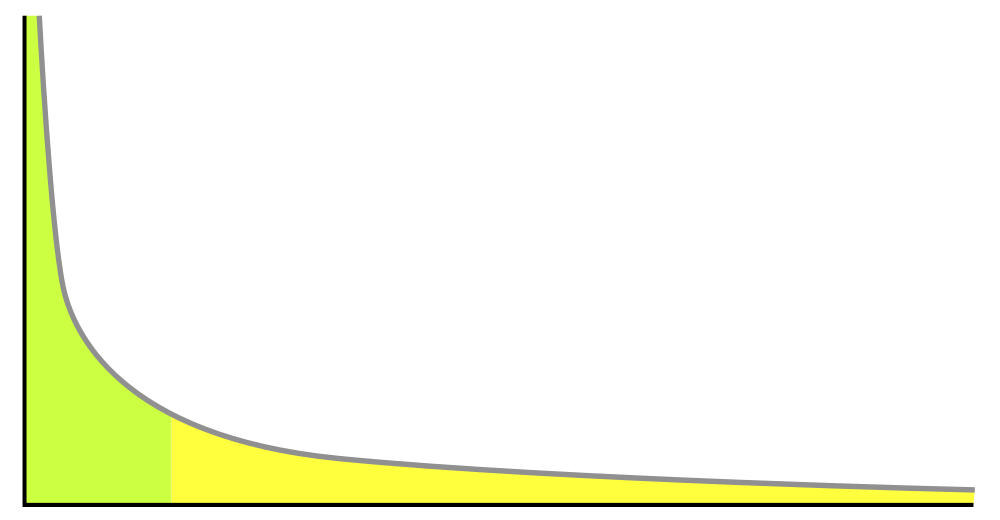
\includegraphics[width=.6\columnwidth]{long-tail.png}
\caption{Uma distribuição de cauda longa. Note que as áreas das duas regiões são iguais, onde a região para a direita representa a cauda longa.}\label{cauda-longa}
\end{center}
\end{figure}

Entretanto, uma quantidade importante de comportamentos da natureza e atividades humanas obedecem a uma distribuição estatística assintótica, conhecida como cauda longa (vide Figura \ref{cauda-longa}). Por exemplo, a maioria dos cães que vemos são de algumas poucas raças (categorias) e a maioria das raças tem poucos cães, isto é são raras. Na indústria existem cada vez mais produtos de nicho. Na Amazon, por exemplo, já em 2008 os produtos de nicho representavam 36.7\% das vendas \cite{erik} e com certeza esse número aumentou nos últimos 10 anos. 

Na indústria de cosméticos uma empresa chega a ter milhares de produtos diferentes (\textit{skus}). Além disso, imagens desses produtos aparecem em diferentes contextos, "domínios": fotos de marketing, que são feitas por fotógrafos profissionais e fortemente modificadas digitalmente para diferenciar e "embelezar" os produtos; e fotos reais que são produzidas por fotógrafos amadores com diferentes equipamentos, condições de iluminação e pose; ou seja, cada domínio tem um viés em termos de variedade visual, como a resolução, \textit{viewpoint} e iluminação.

Essa característica do mundo que nos cerca representa alguns desafios para a aplicação prática dos algoritmos de reconhecimento e classificação: (a) o número de categorias pode ser muito grande, (b) o número de amostras para treinamento pode ser muito pequena\cite{horn} e (c) os domínios das imagens de treinamento e teste podem ser diferentes. 

Neste contexto, bancos de imagens que permitam os algoritmos de reconhecimento a lidar com esses problemas de transferência de domínio e cauda longa são extremamente bem-vindos. 

\subsection{Objetivo}
Este projeto tem dois objetivos: (1) criar um banco de imagens de produtos de cosméticos com amostras de diferentes domínios e (2) ilustrar, com um algoritmo de reconhecimento de objetos, o impacto da mudança de domínio. 

\section{Revisão Teórica}

\subsection{Reconhecimento de Objetos}
Reconhecimento de Objetos lida com a identificação de objetos em imagens. Esta tarefa tão natural aos seres humanos é um grande desafio para algoritmos. Até recentemente, o arcabouço mental para desenvolvimento de algoritmos era a ideia de instruir o computador, passo a passo, como realizar uma tarefa. Mas como ensinar um computador a enxergar? Como instruir, passo a passo, algo que não sabemos como fazemos?

O momento crucial na melhoria meteórica dos resultados em reconhecimento de objetos se deu em 2012, no desafio \textit{ImageNet Large Scale Visual Recognition Challenge}  (ILSVRC)\cite{goodfellow}. O time liderado por Alex Krizhevsky foi o primeiro a usar redes neurais convolucionais profundas (RCPs) na competição e ganhou por larga margem\cite{alexnet}. Desde então, técnicas baseadas em RCPs tem sido as mais bem sucedidas para este problema. É importante salientar, entretanto, que tal feito não seria possível se não houvesse uma banco de imagens de larga escala, manualmente anotada e com centenas de imagens por classe, como a ImageNet.
\begin{figure}[ht!]
\begin{center}
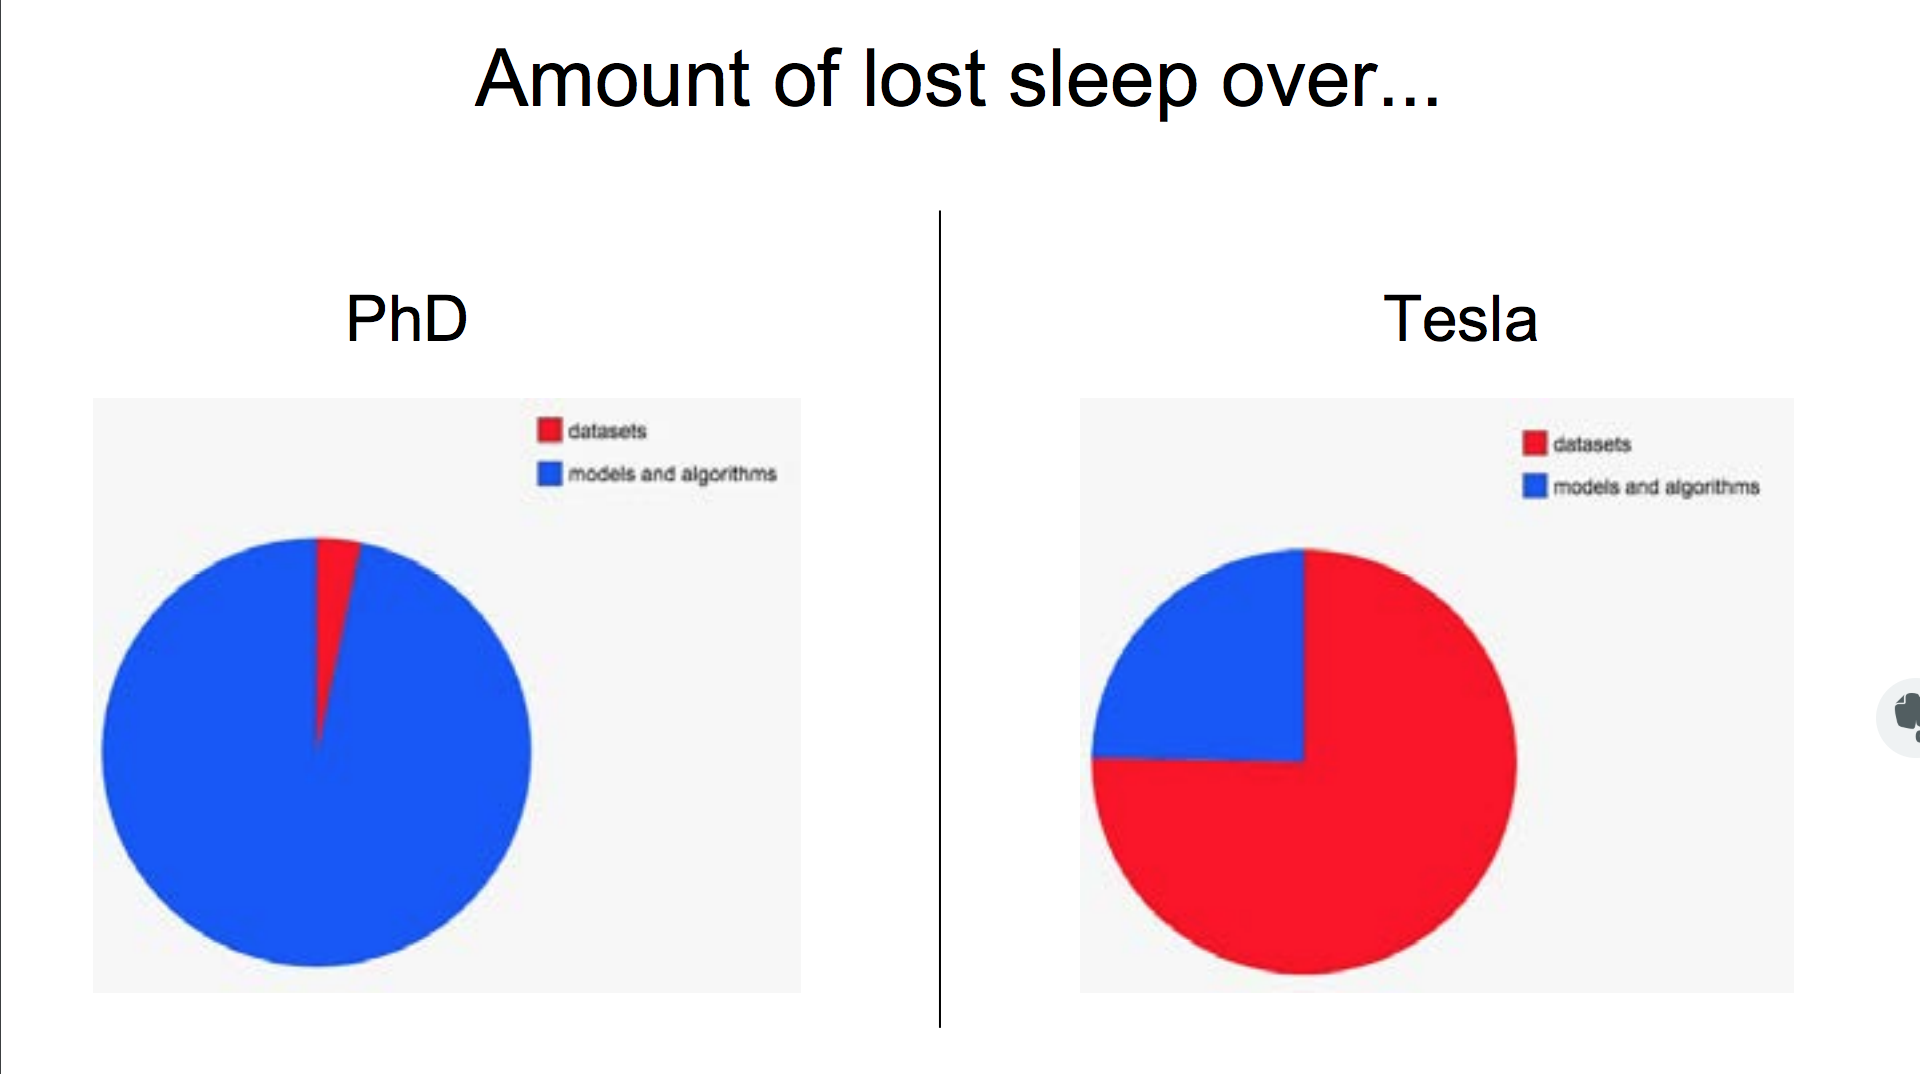
\includegraphics[width=.7\columnwidth]{slide-karpathy.png}
\caption{Diferença entre academia e indústria segundo Andrej Karpathy\cite{karpathy}. (\small{Datasets em vermelho; Modelos e algoritmos em azul.})}\label{slide-karpathy}
\end{center}
\end{figure}
Andrej Karpathy\cite{karpathy} afirma que a maior diferença entre o trabalho como aluno de doutorado em Stanford e como diretor de IA da Tesla é o foco na criação e manutenção de bancos de imagens (Figura \ref{slide-karpathy}). Cada vez mais são os bancos de imagens, e não algoritmos, o fator limitante da aplicação prática e desenvolvimento da inteligência artificial. 

\subsection{Bancos de Imagens para Reconhecimento de Objetos}

Bancos de imagens são vitais para a pesquisa em reconhecimento de objetos. Pode-se dizer que foram um componente chave para o metéorico progresso obtido nos últimos anos, não apenas como fonte de dados para treinamento, mas também como meio de comparação de resultados de pesquisa\cite{bias}. 

Caltech 101 (2004)\cite{caltech} foi um dos primeiros bancos de imagens padronizados para reconhecimento de objetos, com 101 classes de objetos e entre 15 e 30 imagens de treinamento por categoria. O banco de imagens Pascal Visual Object Classes (2006)\cite{pascal}, Pascal VOC, com 20 categorias e imagens obtidas na internet, popularizou a ideia de associar um banco de imagens padronizado com \textit{ground-truth} e uma competição. Fortemente influenciado pelo Pascal VOC, ImageNet (2009) \cite{imagenet} é um banco de imagens organizado de acordo com a hierarquia da WordNet\cite{wordnet}. Apesar das mais de 14 milhões de imagens manualmente anotadas e 21 mil categorias, o subconjunto de sua base destinado à competição ILSVRC, com 1,4 milhão de imagens e apenas 1000 categorias, é mais utilizado. 

\subsection{Viés em Bancos de Imagens e Generalização de Domínios}

Faz pouco sentido esperar ausência de viés em qualquer representação do mundo visual. A maioria dos bancos de imagens se propõe a representar o ambiente visual encontrado no dia a dia das pessoas. Mas é impossível avaliar o quão bem um banco de imagens atende esse objetivo, ou qual é o seu viés, sem ter um \textit{ground truth} (que por sua vez seria uma base de dados que também poderia ter viés)\cite{bias}. 

Pode-se dizer, inclusive, que o desenvolvimento de bancos de imagens se dá através da reação a vieses passados: O banco de imagens COIL-100 (100 objetos comuns em um background preto) foi uma reação ao uso de bases modelo e passou a valorizar texturas. A coleção Corel Stock Photos foi uma reação a simplicidade visual de bases como COIL-100. Caltech-101 foi uma reação ao profissionalismo das fotos da Corel e valoriza a diversidade das imagens da internet. Pascal VOC foi uma reação a inexistencia de padrões de treinamento e teste. Imagenet é uma reação a inadequação de bancos de imagens anteriores que eram pequenos demais para a complexidade visual do mundo\cite{bias}.

Diante deste dilema, uma maneira de se avaliar o viés de bancos de imagens é checar a generalização entre bancos de imagens: por exemplo, treinar com imagens Pascal VOC e testar com imagens da ImageNet\cite{bias}.

Entretanto, a questão da generalização de domínio é tratada como um caso especial do reconhecimento de objetos chamado adaptação de domínio e é menosprezada na grande maioria dos desenvolvimentos de bases de imagens. Praticamente não se encontra comparações de resultados em-domínio (\textit{in-domain}) e entre-domínios (\textit{cross domain}) para os algoritmos baseados em redes neurais convolucionais profundas. 

\section{Metodologia}\label{metodologia}

\subsection{Materiais}
Foram utilizados:
\begin{itemize}
  \item Servidor Paperspace/Fastai: GPU 8GB, 30GB RAM, 8 CPU
  \item NVIDIA Quadro P4000 com 1792 CUDA cores.
  \item Python 3.6.4 :: Anaconda custom (64-bit)
  \item Pytorch 0.3.0
  \item OpenCV 3.4.0
  \item Programa RectLabel
  \item 5 Notebooks Jupyter
  \item 12 programas python.
  \item celular Samsung S8
  \item um pano vermelho de 2m x 1,2m
  \item 168 produtos da empresa O Boticário
\end{itemize}
Todos os arquivos do projeto estão publicamente disponíveis em  \url{git@github.com:fredguth/unb-cv-3183.git}\label{repo}

\subsection{Construção da Base de Imagens}

A base de dados UNBeauty foi construída com dois domínios. Importante mencionar que no domínio das fotos profissionais já dispunhamos de imagens de várias revistas dO Boticário.

\begin{enumerate}
  \item Domínio vídeo de celular
    \begin{enumerate}
      \item Obtivemos 168 diferentes produtos (\textit{skus}) da marca O Boticário;
      \item Montamos uma mesa apoiada em uma parede e pregamos um pano vermelho da parede até cobrir totalmente a mesa;
      \item Com o celular Samsung S8, fizemos um vídeo de poucos segundos (6 a 15s por produto) da parte frontal de cada produto nesse cenário.  Quando o produto era transparente, também fizemos um vídeo do mesmo contra um fundo branco;
      \item Para cada vídeo, anotamos o código do produto e alteramos o nome do vídeo para o nome do código do produto.  Quando mais de um vídeo foi feito para o mesmo produto, simplesmente acrescentamos uma letra (b, c, etc);
      \item Convertemos os vídeos em imagens organizadas por categoria (movie2images.py);
      \item Fizemos uma calibração de cores simples em todas as imagens (balanceDataset.py).
    \end{enumerate}
  \item Domínio das Imagens de Revista
    \begin{enumerate}
      \item Baixamos as imagens das revistas de um repositório S3 (importMags.py);
      \item Com o programa RectLabel anotamos com bounding boxes os produtos para os quais tínhamos imagens no domínio do vídeo de celular;
      \item A partir do json gerado pelo RectLabel, usamos o programa boti-4.py para gerar um dataset chamado mags\_test organizado por categoria.
    \end{enumerate}
\end{enumerate}

Um aspecto importante a salientar é que escolhemos domínios com características bem diferentes. O domínio do vídeo do celular permite várias imagens por classe, mas todas muito similares. O domínio das imagens de revista apresenta poucas amostras por classe e imagens que são bastante modificadas em termos de cores e composição. Esperamos que essa escolha possa ressaltar a diferença da classificação \textit{in-domain} da \textit{cross-domain}.
 \subsection{Classificador de objetos}
O método de reconhecimento de objetos desenvolvido nesse projeto foi fortemente influenciado por \cite{fastai} e constitui-se das seguintes etapas:

 \begin{enumerate}
  \item Definimos Resnet-50 como arquitetura RCP e obter rede pré-treinada com imagens da base ImageNet;
  \item Usando o programa split\_dataset.py, dividimos o dataset em bases estratificadas de treinamento, validação e teste, com 9.084, 2.272 e 2.839 imagens, respectivamente;
  \item Relaxamos as últimas 2 camadas restantes da Resnet-50;
  \item Otimizamos a Taxa de Aprendizado (Learning Rate);
  \item Otimizamos o resultado em Tempo de Teste (Test Time Augmentation)
  \item Rodamos 5 vezes o teste para obter a média e o desvio padrão da acurácia;
  \item Repetimos os passos acima usando a base mags\_test com imagens do domínio das fotos profisionais
  \item Repetimos os passos acima aplicando \textit{Data Augmentation} 
\end{enumerate}
\section{Resultados}
Nesta seção apresentamos os resultados obtidos. Todos os dados podem ser acessados no repositório do projeto (\ref{repo}).
\subsection{Base de Imagens UNBeauty}
Com o método apresentado, obtivemos uma base de dados com:
\begin{itemize}
\item 14.195 imagens de produtos no domínio do vídeo de celular; divididas em
\item 168 categorias, nomeadas pelo \textit{sku} que representavam
\item uma seleção estratificada de treinamento, validação e teste com 9.084, 2.272 e 2.839 imagens, respectivamente;
\item 53 imagens de teste no domínio das fotos profissionais em 45 categorias
\end{itemize}
\begin{figure}
\centering
\subfloat[Linha Coffee]{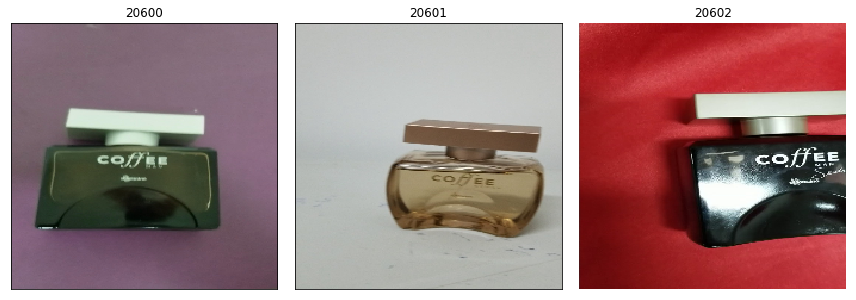
\includegraphics[width=\columnwidth]{coffees.png}}\hfil
\subfloat[Linha Floratta]{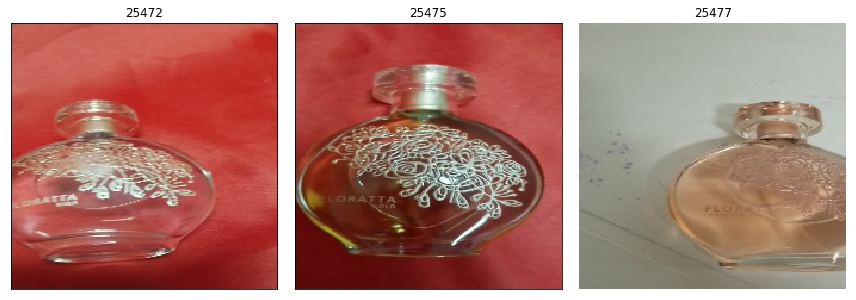
\includegraphics[width=\columnwidth]{florattas.png}}\hfil
\subfloat[Linha Match]{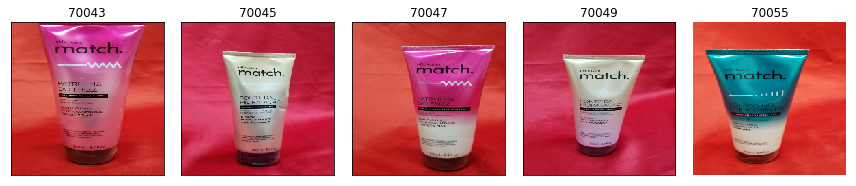
\includegraphics[width=\columnwidth]{matches.png}}
\caption{Produtos de uma mesma linha podem ser bastante similares.}\label{parecidos}
\end{figure}
\begin{figure}[ht!]
\begin{center}
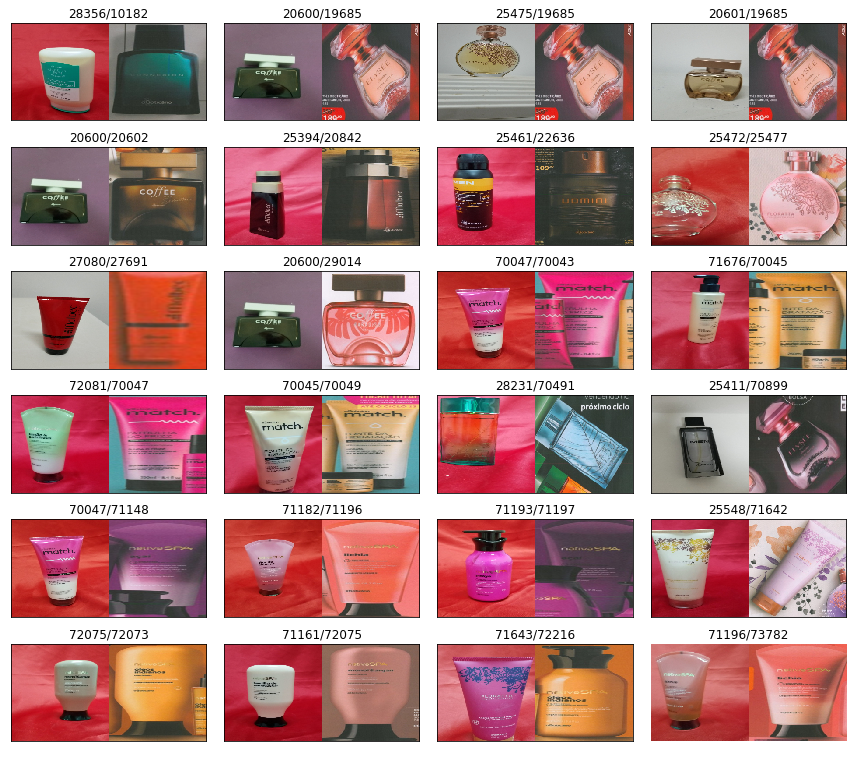
\includegraphics[width=\columnwidth]{erros.png}
\caption{Erros do classificador}\label{erros}
\end{center}
\end{figure}
A base é de alta granularidade, com várias categorias muito parecidas entre si, como mostrado na Figura \ref{parecidos}. A diferença entre os domínios pode ser observada na Figura \ref{erros}.

\subsection{Classificação de Objetos entre domínios}

\begin{table}[]
\centering
\caption{Média e desvio padrão da acurácia ($\phi$) no reconhecimento de objetos}
\label{tabela}
\begin{tabular}{@{}llll@{}}
\toprule
 & Augmentation & $\overline{\phi}\%$ & $\overline{\sigma}\%$ \\ \midrule
\multicolumn{1}{l}{\multirow{2}{*}{In-domain}} & \multicolumn{1}{l}{Não} & \multicolumn{1}{l}{99.89} & \multicolumn{1}{l}{0.05} \\ \cmidrule(l){2-4} 
\multicolumn{1}{l}{} & \multicolumn{1}{l}{Sim} & \multicolumn{1}{l}{99.94} & \multicolumn{1}{l}{0.03} \\ \midrule
\multicolumn{1}{l}{\multirow{2}{*}{Cross-domain}} & \multicolumn{1}{l}{Não} & \multicolumn{1}{l}{47.17} & \multicolumn{1.53}{l}{-} \\ \cmidrule(l){2-4} 
\multicolumn{1}{l}{} & \multicolumn{1}{l}{Sim} & \multicolumn{1}{l}{55.32} & \multicolumn{1}{l}{1.41} \\ \bottomrule
\end{tabular}
\end{table}
Na tabela \ref{tabela}, apresentamos os resultados quantitativos do classificador de objetos. Na figura \ref{erros}, mostramos a natureza dos erros do classificador.
\subsection{Análise dos resultados}

Apesar de servir ao propósito, há alguns problemas na base UNBeauty:
\begin{itemize}
\item o pano de fundo nas imagens do domínio do celular foi uma péssima escolha.  O vermelho é brilhoso, reflete nos produtos e altera a cor dos mesmos, principalmente aqueles mais transparentes. 
\item tentamos sem sucesso melhorar o problema do fundo da imagem de vídeo.  Criamos um classificador de background/foreground inspirado por \cite{ribeiro} usando k-means e aplicando sobre os clusters um criterio bayesiano para definir se o cluster era foreground ou background(GTmaker.py, images2quant.py). Apesar de apresentar um resultado razoável no domínio dos vídeos, o classificador funcionou muito mal no domínio das revistas e acabamos não utilizando as imagens geradas.
\item as imagens das revistas se repetem entre revistas, de forma que foi difícil encontrar amostras diferentes de cada produto.
\item nem todos os produtos do domínio do celular foram encontrados nas revistas. Em retrospecto, teria sido mais eficiente ter primeiro obtido o maior número de amostras diferentes no domínio das revistas e só fazer vídeos dos produtos encontrados. 
\end{itemize}
\subsection{Classificação de Objetos entre domínios}
O classificador de objetos funcionou dentro do esperado:
\begin{itemize}
\item como as imagens do domínio do vídeo são muito parecidas, a acurácia do classificador in-domain foi bem alta, acima de 99\%, falhando apenas entre 2 categorias muito parecidas.
\item no reconhecimento cross-domain a acurácia caiu bastante, praticamente pela metade.
\item um resultado um tanto inesperado foi o fato que aumento de dados melhorou muito pouco o resultado.  Importante salientar que foram tentadas várias técnicas de aumento de dados e em várias delas o resultado foi pior do que sem aumento e estes casos foram descartados.
\end{itemize}

\section{Discussão e Conclusões}
Neste trabalho, desenvolvemos uma base de imagens de produtos de cosméticos com imagens de dois domínios bastante diferentes. Acreditamos que o futuro do desenvolvimento dos algoritmos de reconhecimento de objetos passa por uma maior ênfase na transferência de conhecimento entre domínios. Com uma implementação de um algoritmo de reconhecimento de objetos com redes neurais convolucionais, ilustramos as dificuldades encontradas ao tentar aplicar um algoritmo treinado em um domínio em testes com imagens de outro. Esperamos que a base, com todas as suas imperfeições, possa ser utilizada para ajudar no avanço na direção de algoritmos de reconhecimentos de objetos mais robustos a mudanças de domínio. 

% \begin{figure}[htbp]
% \centerline{
\includegraphics{fig.jpg}}
% \caption{Example of a figure caption.}
% \label{fig}
% \end{figure}

\selectlanguage{brazilian}
\bibliographystyle{IEEEtran}
\bibliography{references}

\end{document}
